\section{Case 1: Resolving Context Ambiguities Using Model Refinement}
\label{contextAmbiguities}
\subsection{Endless-loop Tachycardia}
\subsection{Requirement Encoding}
\begin{itemize}
	\item Pre-condition: Normal atrial self-activation rate (60bpm - 100bpm)
    \item Post-condition: Ventricular pace rate no faster than LRI
\end{itemize}
\Hao{Need a monitor here}
The requirement can be translated to:
$$R1: NA\_self.min=600,NA\_self.max=1000\Rightarrow VP-VP>=TLRI$$
$Prop(R1)=NA\_self$
\subsection{Requirement-guided model refinement}
\begin{Verbatim}
function [HM]=eligible(HM\_tree,Req)
   find HM in HM\_tree with all Prop(Req)
	 while (no parameter in Prop(Req) is merged with other parameters)
	    Go one level up
			endwhile
	 Return HM at current level
\end{Verbatim}
$NA\_self$ is in $H_3$, we go one level up, in $H_4$ the behavior is not merged with any other parameters. In $H_5$ $NA\_self$ is merged with  $NA'-NV'.cond$ so $H_4$ is returned as the appropriate heart model for R1. In \cite{STTT13} we used $H_4$ to verify the correctness of the ELT termination algorithm. With a basic DDD pacemaker we have $H_4 || P_{DDD}\models R1$. The counter-example returned is exactly the ELT behavior. Then we implement the ELT termination algorithm and we have  $H_4 || P_{ELT}\not\models R1$, meaning ELT has been successfully terminated, and only the ELT is terminated. 

\subsection{Inappropriate Model Refinements}
If we follow the traditional CEGAR framework and verify the property using $H_5$, an abstract counter-example would return, which is shown in \figref{C_amiguity}. However the counter-example correspond

\begin{figure}[!t]
		\centering
		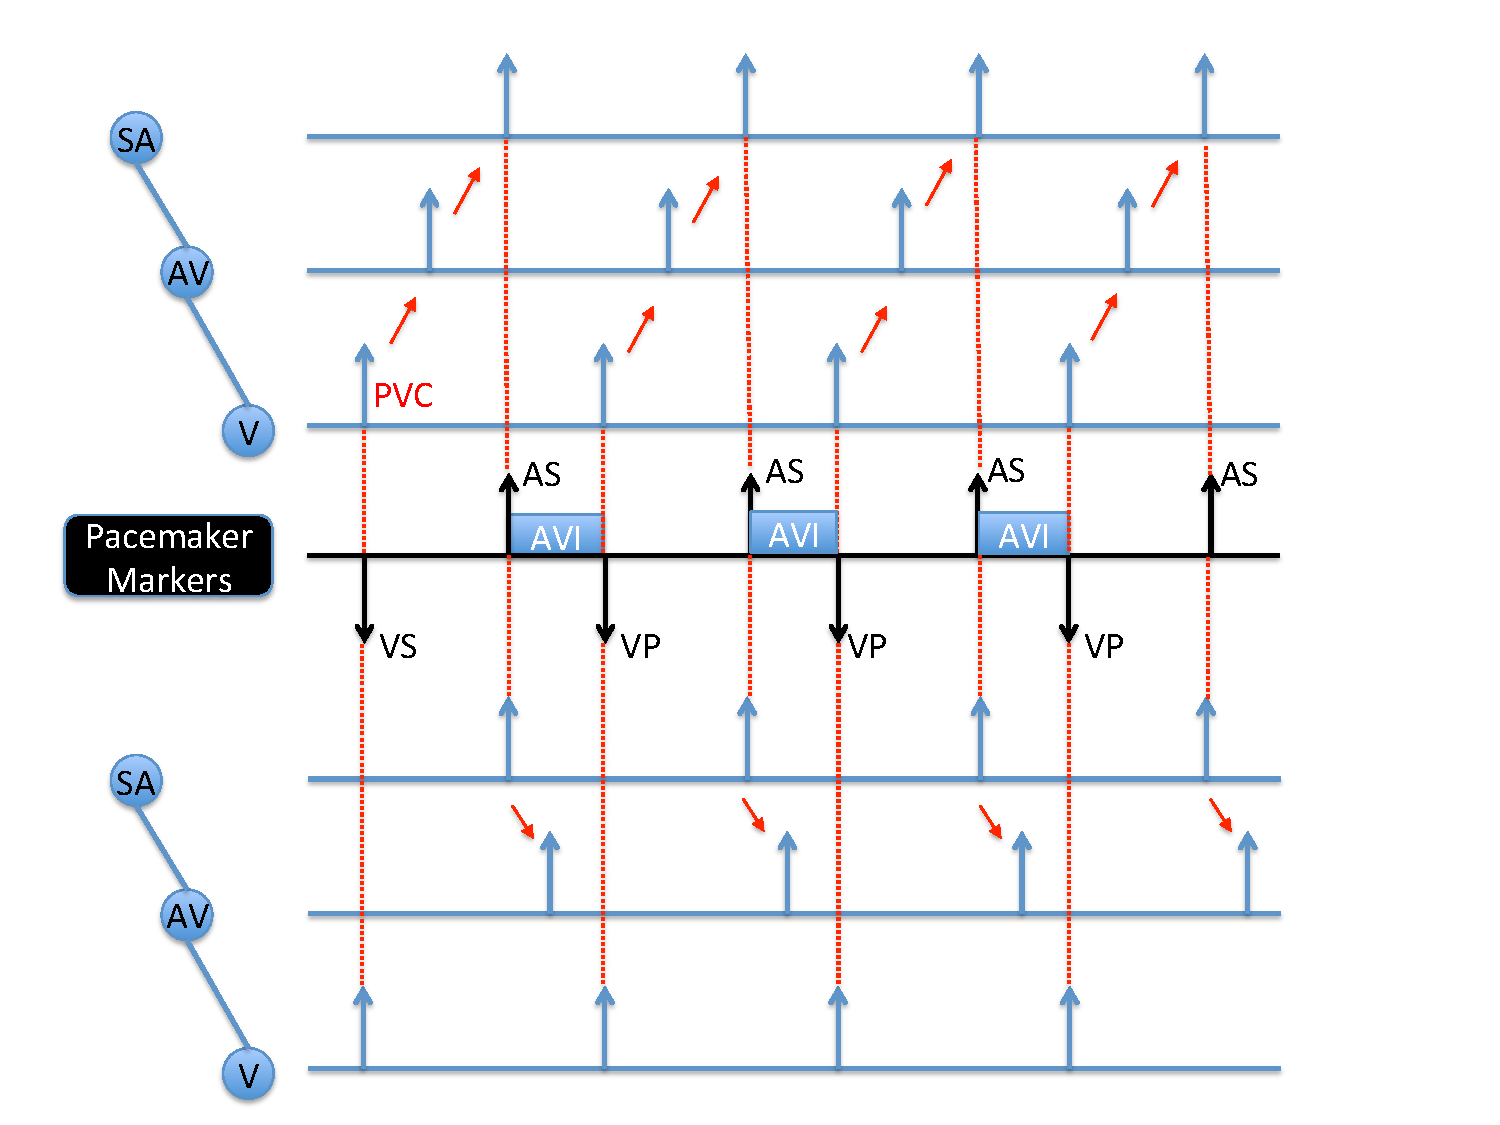
\includegraphics[width=0.8\textwidth]{figs/ambiguity.pdf}
		%\vspace{-5pt}
		\caption{\small Heart Model Abstractions}
		  %\vspace{-15pt}
		\label{fig:C_ambiguity}
\end{figure}



